\chapter{Introduction}\label{introchapter}
Among sensory systems, the auditory system is perhaps the most ubiquitous. The 
development of numerous strategies for the detection and processing of auditory stimuli
across several species is a testament to this fact; cf. Sec. \ref{auditoryevolution}. The processing of sound stimuli is fairly fast and in comparison
to light stimuli, sound has two main properties - it is omnidirectional and due to
its large wavelength it isn't blocked by small objects. For instance we can hear objects
behind us or behind obstacles whereas the same isn't true for visual stimuli. These properties 
give the animal the obvious advantage of being able to react to approaching dangers that
aren't yet visible. In order to fully utilize the sound stimuli, it is therefore essential
that an animal is able to assess the direction or, to use the technical term, \emph{localize} a sound source.

Before we discuss the various sound localization methods observed in nature, we first
go through the fundamental steps involved in auditory perception. First, an object generates
an auditory stimulus which in general can be very complex. This stimulus then propagates
through a given medium (e.g. air, water) and excites the primary receiver(s) of the animal. In most
terrestrial vertebrates, these take the form of \emph{tympani} or eardrums - a pair of thin vibrating
membranes which are a component of the mechanical part of the auditory system.
Depending on the species, there may be an apparatus that focuses and amplifies the sound waves. In
humans for example, this function performed by the external ears or pinnae. 
The vibrations are then transmitted by means of a set of bony or cartilaginous elements and
converted into electrochemical signals that will be processed neuronally; see Sec. \ref{mechanicalprocessing}.

The neuronal processing system consists of building blocks called \emph{neurons} which are
connected to each other through \emph{synapses}. The entire system is referred to as a 
\emph{neuronal net} which, through a form of computation, gives rise to representations of the stimuli
known as \emph{neuronal maps}. Each neuron of the map represents a specific property, e.g.
the position in space or the frequency of the stimulus and neighbouring neurons respond to
similar sensory inputs. Neuronal maps serve to reconstruct stimuli as optimally as possible
within the limits of processing. The precise calibration of the
synapses required for stimulus reconstruction is a result of experience-based learning
processes that take into account inputs from all available sensory systems.

The primary focus of this thesis is the mechanical processing that is responsible for the
sound localization ability of certain terrestrial vertebrates. Specifically, we are interested
in the analytical treatment of hearing in animals that have their eardrums connected through a large mouth cavity and the
 enhancement of directionality in the response of such systems;see Sec. \ref{iceintrosection}. Although our model can be scaled to several different species,
 for the purposes of a thorough comparison, we will be putting a special emphasis on lizard hearing. The questions posed by the neuronal processing of auditory stimuli in these
animals although interesting, are beyond the scope of this thesis. However, in order to have a basic understanding of the neuronal basis for our analysis, we will briefly discuss the neuronal processing of the binaural cues
in these animals in Sec. \ref{iceneuro}.

\section{Mechanical Processing of Auditory Stimuli}\label{mechanicalprocessing}
\subsection{Evolution of Different Auditory Systems}\label{auditoryevolution}
Ancestors of most modern vertebrates including frogs, turtles, lizards, birds, crocodilians and mammals
developed a pair of tympani (thin vibrating membranes) to detect incoming sound waves and transmit
them from the air to the ossicles in the middle ear; cf. Fig. \ref{vertebrateearevolution}. 
Despite the large variation in size and shape, two groups with fundamentally distinct constructions can be
made out. Mammals posses tympani that are effectively separated from and therefore acoustically 
independent of each other. In contrast, the other group consisting of reptiles (lizards, turtles, crocodiles), birds and frogs
have \text{Internally Coupled Ears} (for reviews see \cite{carrsoares}, \cite{dalsgaardcarr} and \cite{schnuppcarr}) wherein
the tympani are connected through large Eustachian tubes as illustrated in \ref{lizardheadcrosssection}. The evolutionary 
appearance of independent and coupled ears (Fig. \ref{vertebrateearevolution}) suggests that the latter are probably early
tympanic ears.
\begin{figure}[ht!]
 %\centering
 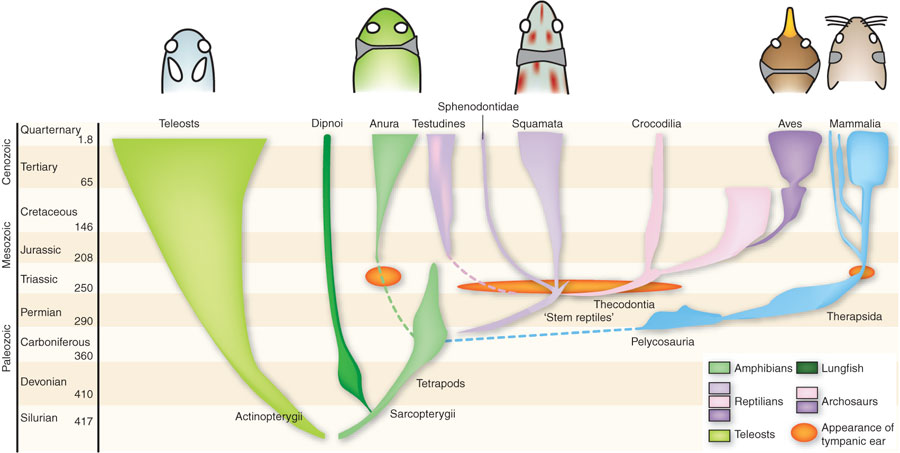
\includegraphics[width=1.0\linewidth]{Diagrams/vertebrateearevolution.jpg}
 \caption[Vertebrate Ear Evolution]{Evolution of vertebrate ears. Tympanic
 middle capable of receiving airborne sound evolved independently among the ancestors of modern frogs, turtles, lizards, birds,
 crocodilians and mammals. Diagrams at the top show cross-sections through different heads of these animals (middle ears - gray fill).
 Among these middle-ear systems two distinct groups can be observed - the anura (frogs and toads), squamata (lizards and snakes)
 and aves (birds) form one group with ears connected through differently shaped cavities and mammals with independent ears. Figure due to Schnupp and Carr \cite{schnuppcarr}.}
 \label{vertebrateearevolution}
\end{figure}

\begin{figure}[ht]
 \centering
 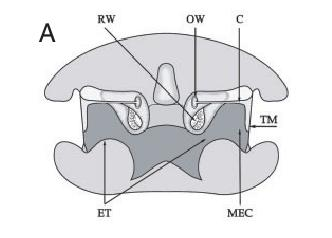
\includegraphics[width=0.45\linewidth]{Diagrams/lizardheadcrosssection.jpeg}
 \caption[Cross Section of a Lizards Head]{Diagram of the cross-section of a lizard’s head (\emph{sceloporus}). The Tympanic Membranes (TM) as well as
 the air inside the Middle Ear Cavity (MEC) and Eustachian Tubes (ET) are excited by incoming sound waves. Due to the considerable width of the Eustachian Tubes (ET), the air inside the Pharynx (P) is excited as well.
 The vibration of the tympanum causes a movement of the attached middle ear, Columella (C) whose lever construction transmits the vibrations to the Oval Window (OW), the membrane at the entrance of the fluid filled cochlea.
 Figure taken from \cite{dalsgaardmanley1}. The vibration of the OW excites the fluid in the Cochlea which gives rise to a frequency-dependent activation of the embedded basilar membrane and underlying
 auditory nerve fibers. The Round Window (RW) is a membrane at the end of the cochlea that serves to compensate the pressure within the fluid.}
 \label{lizardheadcrosssection}
\end{figure}

\subsection{Pressure Difference Receiving Ears - The ICE Model}\label{iceintrosection}
The ability of humans and most other mammals to localize sources of sound depends on two kinds of information: the direction and frequency
of the source may cause differences between the amplitudes (ILDs -Interaural Level Differences) and arrival times ((ITD -Interaural Time Differences) of sounds reaching both ears. These pieces of information are
referred to binaural hearing cues or simply hearing cues. In mammals there is an additional source of directionality due to the shape
of the pinnae which affects the spectra of sounds reaching the ear (monoaural cues). In effect, the ears are independently activated by sound pressures
on their external surface. In humans, at frequencies above $1.5$kHz, the amplitude differences between the eardrums are sufficient
to localize the source whereas at lower frequencies the time cues are mainly used. The amplitude cues are a result of the ear farther
from the source being in the 'sound shadow' of the head due to diffraction effects. The time cues are a result of the sound having to travel
different paths to reach either ear and is in general not as strongly affected by diffraction.

However, most hearing animals are lack monoaural cues and the binaural
cues are at best too small to affect the neural responses of the ears, \cite{michelsen1}. These animals are in general too small in comparison
to the wavelength of sound in their typical hearing range to cause an appreciable amplitude differences due to diffraction. Nevertheless, 
the eardrum vibration amplitude has been found to vary strongly with direction. In order to resolve this apparent paradox it was
suggested by Autrum \cite{autrumjcomphys} that in locusts the directionality could be a result of the ears vibrating due to the
differences between the pressure on the inner and outer surfaces (see \cite{michelsenlarsen} for a review).  The properties of such systems were also found to be analogous with the inherently directional 
nature of pressure gradient receivers studied by Harry Olson (\cite{olsonmichrophones}). Pressure difference reception has
become the standard explanation for directionality in almost all small animals; the one exception being mechanically coupled
eardrums in some parasitic flies, (see Robert \emph{et al} \cite{roberthoy}).

The pathway for sound to the inner surface of the eardrum varies. In many animals the air spaces behind the eardrums are
connected by sizable air-filled passage which results in a coupling between the eardrums. This has been shown for 
insects (\cite{michelsenbiophysics}), frogs (\cite{jorgensenanurans}) and reptiles (\cite{dalsgaardmanley1}). The sound wave
may alternatively reach the inner surface of the eardrum through a different route (like the tracheal tube in crickets). Our focus
is on the construction and mathematical analysis of a model for the former type of animals, i.e. animals that have their eardrums coupled through an air-filled cavity. 
The ICE model seeks to explain the emergence of enhanced directional cues in animals that are small relative to wavelengths
in their entire hearing range. As a result, they are forced to exploit the small time differences between the inputs between
their ears to localize a sound source. Using these small ITDs, the system generates amplified
 time differences (which we will refer to as iTDs - Internal Time Differences) and direction dependent amplitude differences (which we will
 refer to as iLDs - Internal Level Differences) between the tympani.
 
The primary advantage of pressure difference receiving ears is to compensate for a small body size relative to sound wavelengths. It has
however also been suggested that there is another reason for this adaptation. The natural habitats of such animals
is usually close to the ground resulting in a severe degradation of directional cues due to the presence of obstacles. Amplitude cues are especially affected due to multiple reflections and other deviations
from a free sound field. In contrast, the contribution to the scatter of phase cues due to diffraction are not nearly as dramatic (the degradation
of these cues for a grasshopper in its natural grassland habitat was studied my Michelsen and Rohrseitz \cite{michelsenrohrseitz97}). Therefore,
 by only exploiting phase cues, these animals would have a much more accurate localization strategy than by exploiting amplitude cues. Moreover, 
 the scattering of both amplitude and phase in dense habitats increases with frequency suggesting that animals in these habitats should prefer to
 use rather low frequencies for communication. 

Following Vossen \cite{vossenjasa},  we refer to our model as ``ICE'' (Internally Coupled Ears). Our goal is to analyse the physics behind the production of the
enhanced differences (iTD/iLD). In particular we are interested in the frequency and direction dependence of the hearing cues. The problem of
directional hearing in lizards was previously treated by Vossen (see Chapter 2 of \cite{vossenthesis} and Vossen \emph{et al} \cite{vossenjasa}).
Here, an analytical model of internally coupled ears with a cylindrical air cavity was first presented. This thesis aims to be an extension of the previous work
wherein we seek to provide an analytical model that reflects the frequency and directional behaviour of such systems in nature. Our work deviates in
the treatment of the following aspects - 
\begin{itemize}
 \item While constructing the mouth cavity we place an emphasis on maintaining its volume resulting in different radii for the tympanum and the cylindrical cavity; See Sec. \ref{subsecinnercavity}.
 \item For the pressure inside the cavity (See Sec. \ref{internalcavity}) we propose a different set of modes that represent it more accurately.
 \item The treatment of the membrane and its transducer - the extracolumella (See Sec. \ref{tympanicmembrane}). We propose a construction that is easier to treat analytically and reproduces
 the vibration patterns fairly well.
 \end{itemize}

\section{Neuronal Processing of Hearing Cues}\label{iceneuro}
The neuronal processing of auditory signals starts after the tympanic vibrations are transmitted by the columella (the middle ear bone that is attached to the tympanum)
to the oval window, a membrane at the entrance of the cochlea; see Fig. \ref{lizardheadcrosssection}. The vibration of the oval window results in the vibration of
the fluid within the cochlea and of the embedded basilar membrane. The basilar membrane has a systematically varying stiffness resulting in each of its parts 
reacting to a specific frequency. Auditory nerve fibres that respond to a small range of frequencies do so by being enervated by the movement of specific
regions of the basilar membrane. In this manner, the basilar membrane functions to decompose sound frequencies.

Early stages of auditory pathways in birds and mammals contain synaptic relays designed to preserve the temporal fine structure of 
acoustic stimuli with great accuracy.  Studies of neural processing in Tokay geckos have also shown similar properties \cite{dalsgaardtangcarr}.
These animals possess cochlear nuclei (the collections of neurons that receive input from the cochlear nerve) that are specialized either for
the computation of time differences (iTD/ITD) or level differences (iLD/ILD) between the tympani. The neurons sensitive to level difference are excited by the 
input from one ear and inhibited by the other. These neurons are for obvious reasons known as 'EI' neurons and respond most strongly when the
sounds come from the excitatory ear. The inhibitory ear, on the other hand sits on the far side of the head resulting in an increased firing
rate of the neurons due to reduced inhibition. Similarly, as the sound source moves closer to the inhibitory ear, the neural firing rates decline
due to increased inhibition. Thus, the neural firing rate encodes the sound source position. 

In contrast, the neurons sensitive to time differences are excited by inputs from both ears ('EE' neurons, Fig. \ref{EEtypedetector}a). The strength of the
excitation depends on the exact relative timing of the inputs. Just as is the case for larger animals, the level
differences are more pronounced are most effective at higher frequencies and the time difference cues at lower frequencies. Sound waves are encoded
by neurons as sinusoidal membrane potentials. The primary sensory neurons, known as afferent neurons, phase lock to the input
stimulus and are most likely to fire near the peak of the sound wave. Their synaptic potentials (formed due to differences
in ion concentration) sum to produce fluctuating membrane potentials which resemble the stimulus waveform; see Fig. \ref{EEtypedetector}b. 
\begin{figure}[ht!]
 \centering
 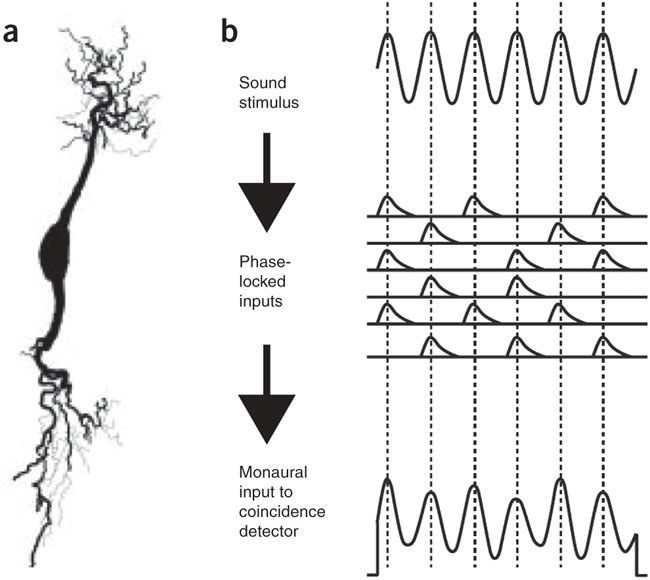
\includegraphics[width=0.7\linewidth]{Diagrams/EEtypedetector.jpg}
 \caption[EE-type coincidence detector and encoding of sound waves as membrane potentials.]{(\textbf{a}) Anatomy of an 'EE-type'
 coincidence detector neuron. Sound signals from both ears converge through the two prominent dendrites (the hair like extensions
 on either end). (\textbf{a}) Encoding of sound waves as sinusoidal membrane potentials. Nerve fibers phase lock to the sound stimulus and
 are therefore most likely to fire near the peaks. Their excitator synaptic potentials sum to produce membrane potentials which resemble the
 stimulus waveform. Figure taken from \cite{schnuppcarr}.}
 \label{EEtypedetector}
\end{figure}

The neurons responsible for 
the processing of time difference queues were classically thought to be organized in a 'delay line and coincidence detector' arrangement, commonly
known as the 'Jeffress model'\cite{jeffressmodel}. According to this model, the firing of individual neurons is response to precisely synchronized excitation
from both ears, and systematically varied axonal conduction delays along the length of the nucleus serve to offset ITDs. Thus each neuron is tuned to a 
specific time delay value that cancels the signal delay from the left and right ear; see Fig. \ref{jeffressmodel}. The appeal of the Jeffress model lies in the elegant way it converts systematic variations in the iTD/ITD into
a topographic map of the sound source location. Initial experimental evidence from birds (\cite{carrkonishi}, \cite{parksrubel}) provides strong support 
for the existence of such a delay line arrangement.
\begin{figure}[ht!]
 \centering
 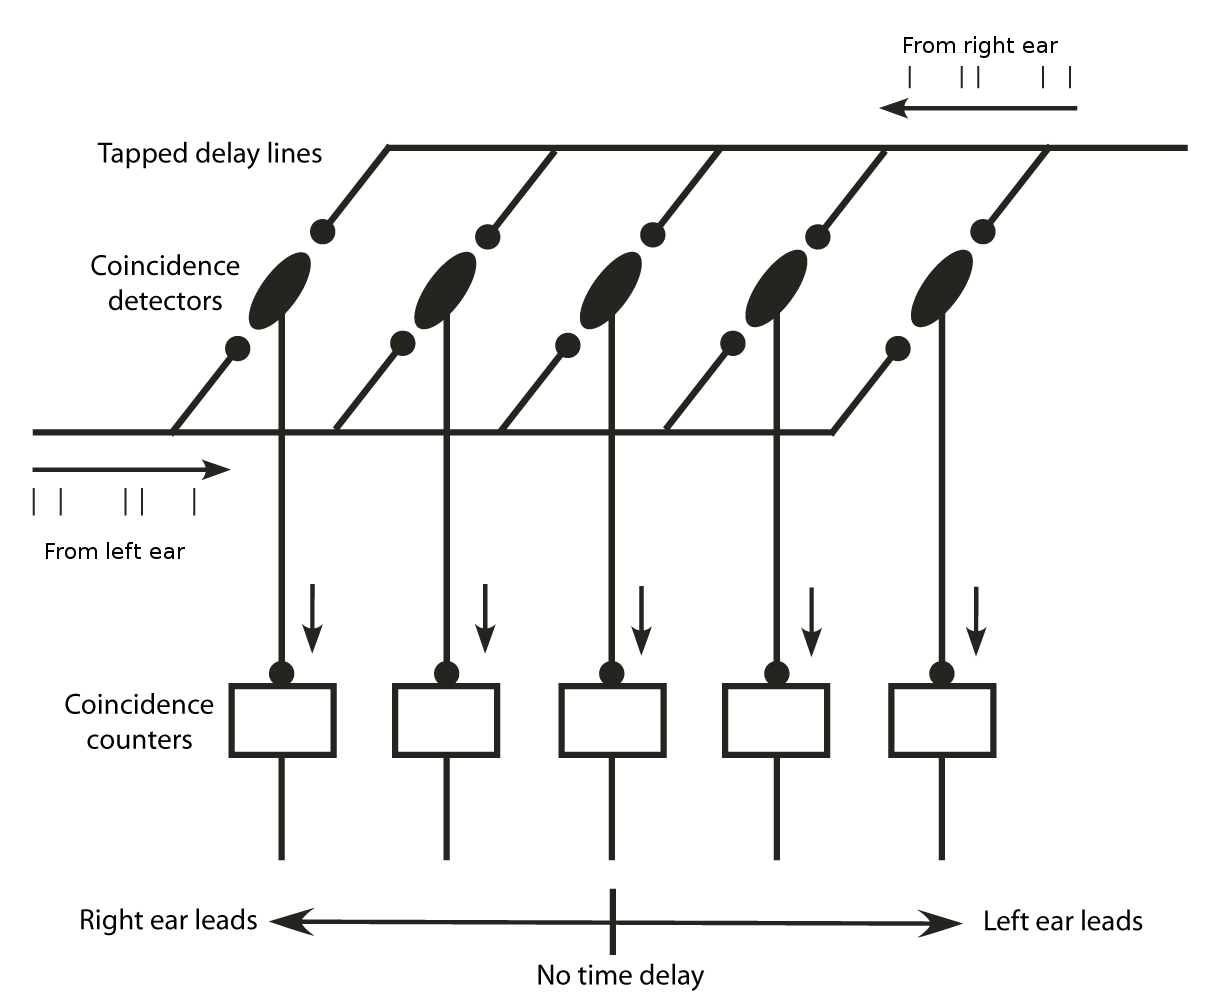
\includegraphics[width=0.6\linewidth]{Diagrams/Jeffress.png}
 \caption[Delay line coincidence detector - Jeffress model]{A very simplified schematic representation of the Jeffress model. The coincidence detector neurons ('EE-type')
 simultaneously receive inputs from both ears through different delay lines. The coincidence counters fire when the inputs to the detectors are synchronized. For
 example when a sound reaches the left ear first, the inputs reaching the rightmost detectors are more synchronized due to the signal from the left ear being
 delayed.}
 \label{jeffressmodel}
\end{figure}

\section{Overview}
Our study will take place in two main steps. In Chapter \ref{modelchapter} we will
present our model for the mechanical processing of auditory signals in systems with internally coupled ears - the ICE Model.
Since our focus is on an analytical model, we would like to have a system that reduces to tractable mathematical expressions
so that we can clearly see the dependence of the system's behaviour on its parameters. To this end we will model the 
combination of the Eustachian tubes, middle ear cavity and pharynx as a single continuous cylindrically shaped air cavity; see
Sec. \ref{subsecinnercavity}. The ears will be modelled as linear elastic membranes that are circular with an omitted sector replaced
by a non-moving plate
that corresponds to the extracolumella - the extension of the columella that is in contact with the ear. The
sound inputs to both the ears will be modelled as pressure waves of a given frequency with a phase difference corresponding to the azimuth of the object that depends on the 
head size and frequency. The aim of the chapter is to find expressions for the quantities which give us the directional output of the system.

In Chapter \ref{modelanalysis} will evaluate the validity of our model
by comparing the calculated values of the membrane vibration velocity with experimentally determined quantities; 
see \ref{vibvelocity}. In addition to testing the directional frequency
response of the system we will also define quantities that could serve as directional cues. These two quantities are known
as the iTD (\emph{Internal Time Difference}) which measures the delay between the membrane vibrations and the iLD (\emph{Internal Level
Difference}) which measures the difference in their vibration amplitudes; Sec. \ref{hearingcuessection}. These quantities are defined in contrast to the
\emph{Interaural} Time and Level  Differences which serve as directional cues in the absence of coupling. Due to the difficulty of measurement of certain membrane
properties (e.g. fundamental frequency, damping coefficients), in Sec. \ref{parameterestimation} we will also provide means of estimating these quantities from observations.
In the final section of this chapter, Sec. \ref{vibrationpatternchapter}, we will compare the vibration profile of our model tympanum with that of a realistic tympanum and thereby
seek to explain the complex patterns of the observed.
